\section{Scope of Work}

\subsection{Initial Situation}
In computer graphics, especially in games, an astonishingly large group of features are reccurring across all programs and genres.
With the most obvious ones being water surfaces, cloudscapes and fire effects, they are present in almost any game. 
Naturally, those features grew in complexity, customizability and computational demands over time.
\\
One of the core mechanics for achieving realistic results is called a \emph{\gls{volumetric} \gls{shader}}.
A prototype such a \gls{shader} has been created in a previous project and will be used as base.

\subsubsection{Previous Work}
In a previous project, the process of creating a \gls{volumetric} \gls{shader} has already been researched and implemented in a prototype. Thanks to its high flexibility, different cloudscapes could be rendered by the same shader.

\begin{figure}[ht]
    \centering
        \begin{minipage}{0.47\linewidth}
            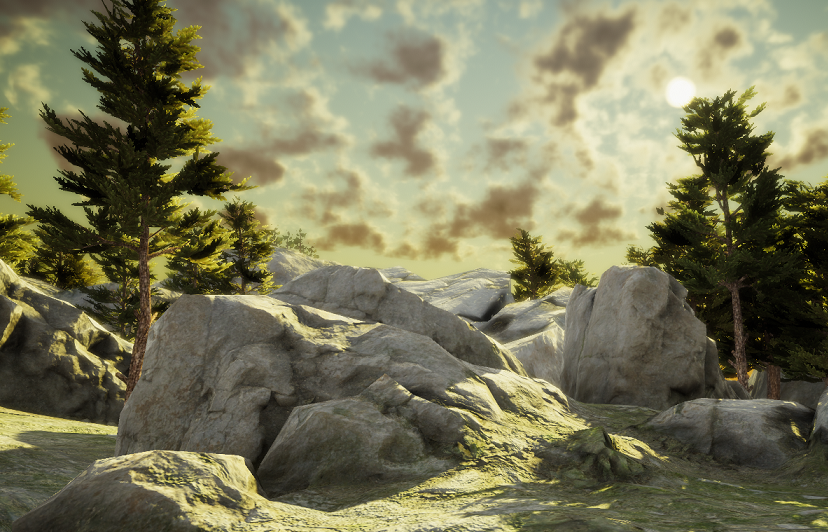
\includegraphics[width=\linewidth]{project2/project2-final.PNG}
            \captionof{figure}{Result of the previous work's shader (Evening).}
        \end{minipage}
    \hfill
        \begin{minipage}{0.47\linewidth}
            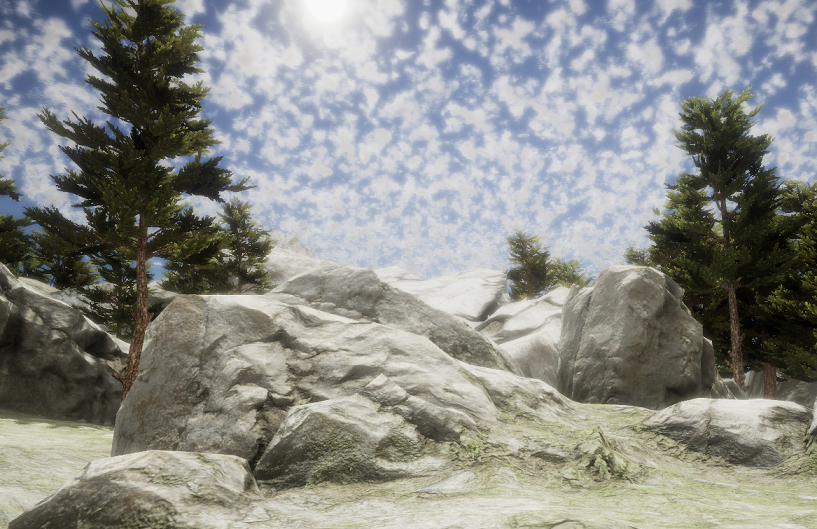
\includegraphics[width=\linewidth]{project2/project2-final2.PNG}
            \captionof{figure}{Result of the previous work's shader (Day).}
        \end{minipage}  
\end{figure}

\noindent
During that project, some other important topics have been researched. Among those were \gls{volumetric} rendering, Perlin and Voronoi \gls{noisegeneration} algorithms, and a technique called \emph{\gls{raymarching}}.
\\
The implementations of those algorithms and methods will most likely be reused in this thesis and will be adapted and improved accordingly.

\begin{figure}[H]
    \centering
        \begin{minipage}{0.47\linewidth}
            
\includegraphics[width=\linewidth]{project2/fbm10_1.png}
            \captionof{figure}{A generated noise texture with Voronoi's algorithm.}
        \end{minipage}
    \hfill
        \begin{minipage}{0.47\linewidth}
            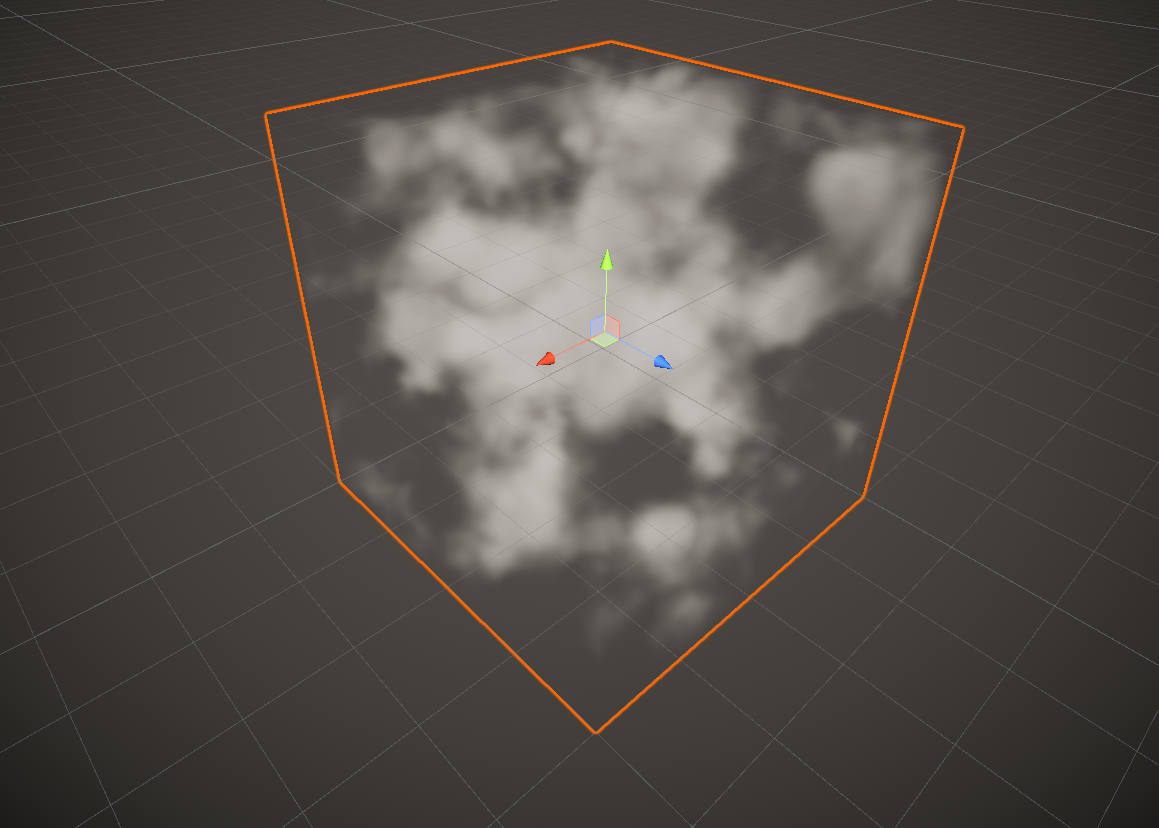
\includegraphics[width=\linewidth]{project2/prototype3.PNG}
            \captionof{figure}{A screen capture of an image rendered with \gls{raymarching}.}
        \end{minipage}  
\end{figure}

\subsection{Goals}
\label{section:goals}
As the title of the thesis suggests, this work will primarily focus on clouds and cloudscapes.
The primary goal of the project is to research and implement rendering techniques for a real-time \gls{procedural} weather rendering system.
\\
The goals will be split into two distinct groups: mandatory and optional. However, this section only defines high-level goals. A detailed specification of all requirements can be found in \sectionref{section:requirements}.

\subsubsection{Mandatory Goals}
The following tasks must be accomplished during the project:
\begin{itemize}
    \item Understanding the basic nature of clouds
    \item Understanding of different layers of clouds
    \item Understanding of compute shaders
    \item Implement a weather rendering system
    \item Incorporate real-time weather data from \emph{meteoblue}
    \item Incorporate topological landscape models from \emph{swisstopo}
\end{itemize}

\subsubsection{Optional Goals}
For further optional work, these tasks can be looked into:
\begin{itemize}
    \item Automatic validation of realism of rendered cloudscapes
    \item Automatic comparison of rendered cloudscapes and photographs
    \item Automatic categorization of rendered cloudscapes
    \item Performance optimization
\end{itemize}

\noindent
Most of the tasks labeled with "automatic" could be solved using a \gls{neuralnetwork}.
As for performance optimization, it is meant to optimize shader code, find early exits for looping algorithms and reduce the overall workload of importing the external data into the weather rendering system.

\subsection{Educational Objectives}
Educational objectives include \gls{shader} programming, knowledge about \gls{computeshader}s, rendering techniques, common algorithms used in computer graphics like \gls{noisegeneration}, a general understanding of aspects needed to create a complete weather system and finally the incorporation of real-time data from a third party.

\subsection{Used Software and Tools}
All documentation will be written in \gls{latex} with Visual Studio Code.
The \gls{shader} will be implemented in Unity. The chosen \gls{shader} language is \gls{hlsl}.
For the presentation, Microsoft PowerPoint will be used.